\documentclass[ä5paper, 11pt]{article}
\usepackage[utf8]{inputenc}
\usepackage{xcolor}
\usepackage{listings}
\usepackage{graphicx}
\usepackage[lmargin=3cm,rmargin=2.5cm,tmargin=2cm,bmargin=2cm]{geometry}
\usepackage{multicol}
\usepackage[export]{adjustbox}
\usepackage{dirtytalk}
\usepackage{float}
\usepackage{fancyhdr}
\pagestyle
\centering{\title {\textbf{\huge \textcolor{red}{Raised by Wolves}}}}

\author{Ivan Borjas }
\date{22 de septiemre de 2022}

\begin{document}
\pagestyle{fancy}
\pagecolor{blue}
\lfoot{Jorge Ivan}
\rhead{\thepage}
\lhead{\lefttmark}
   \centering{\textbf{\huge \textcolor{red}{Rysed by Wolves}}}
   \section*{Elementos generales de la serie}
        \subsection*{Reseña}
     {Después de que la tierra fuera destruida por una guerra entre mitraicos y ateos, Padre y Madre, dos androides fueron mandados a kepler-22b con el fin de criar hijos humanos que posteriormente creen una nueva civilización atea, pero esta mision se ve afectada por conflictos como la alimentacion, los seres que habitan allí ylos mitraicos}
        \subsection*{Elenco}  
          \subsubsection*{Guionistas}
              \begin{enumerate}
              \item [*] {Karen Campbell}
              \item [*]{Heathher bellson}
              \item[*]{Donald joh}
              \item[*]{Aaron Guizikowski}
           \end{enumerate}
          \subsubsection*{Porudctores}
            \begin{enumerate}
                \item[*]{Jon kuyper}
                \item[*]{Jordan Sheehan (productor delgado)}
                \item[*]{ Mark W. Zucker (productor delgado)}
                \item[*]{Ridley Scott (productor delgado)}
                \item[*]{Aaron Guizkoeski (productor delgado)}
                \item[*]{Adam Kolbrenner (productor delgado)}
            \end{enumerate}
          \subsubsection*{Directores}   
             \begin{enumerate}
                \item[*]{Ridley Scott}
                \item[*]{Alex Gabasii}
                \item[*]{James Hawves}
                \item[*]{Sergio Mimica}
                \item[*]{Luke Scott}
            \end{enumerate}
        \subsubsection*{Personajes}
            \begin{enumerate}
                \item[*]\fcolorbox{green}{black}{\textcolor {white}{Amanda Collin (Madre)}} Es la madre de los humanos que nacen en Kepler a pesar de no ser humana parece que siente amor por los niños. A medida que pasa el tiempo y descubre que es un arma que fue modificada para criar niños.
                \item[*]\fcolorbox{black}{black}{\textcolor {white}{Abukar Sakim (padre)}} Es el papá de los niños, se encarga de cuidarlos y proveer alimento, a pesar de que es un androride de servicio siente celos y amor porlos niños, lo que generá la pregunta, ¿imitan las emociones o en reaidad son capaces de sentir?.
                \item[*]\fcolorbox{green}{black}{\textcolor {white}{Winra McGrath (Campion)}} Es el ultimo de los niños que nacieron en Keppler que sigue vivo, como es el ultimo niño ateo no tiene esperanzas de sobrebvir. 
                \item[*]\fcolorbox{green}{black}{\textcolor {white}{Travis Fimmel (Marcus)}}Papá Paul, es un ateo que se infiltra con los mitraicos para sobrevivir, se la pasa fingiendo se un general y el papá de Paul, a pesar de que no es su hijo lo llega querer como si fuera
                \item[*]\fcolorbox{green}{black}{\textcolor {white}{Niamh Algar(Sue)}} Mamá de Paul, al igual que Mrcus se infiltra con los mitraicos para sobrevivir, sucede lo mismo con Paul, aun que apesar de que no es su hijo lo quiere.
                \item[*]\fcolorbox{green}{black}{\textcolor {white}{Felix Jamieson (Paul)}} Hijo de Sue y Marcus, no sabe que sus papás estan muertos, es raptado por madre e intenta volver con sus papás
                \item[*]\fcolorbox{green}{black}{\textcolor {white}{Asiya Shah (Holly)}} Personaje secundario que pertenece a los mitraicos, es la unica de los mitraicos que quiere quedarse con Madre a pesar de que son ateos, es la más chica de los niños raptados
                \item[*]\fcolorbox{green}{black}{\textcolor {white}{Ivy Wong (Vita)}} Personaje secundario que pertenece a los mitraicos
                \item[*]\fcolorbox{green}{black}{\textcolor {white}{Loulou (Taylor)}} Personaje secundario que pertenece a los mitraicos
                \item[*]\fcolorbox{green}{black}{\textcolor {white}{Ethan Hazzard (Hunter)}} Personaje secundario que pertenece a los mitraicos
            \end{enumerate}
    \section*{¿Por qué me gusta?}
        \subsection*{Razones}
          \textcolor{red}{suelo ser indeciso al escoger algo para ver, empecé a ver la serie piorque tenía 3 meses de vacaiones y tenia que hacer algo jaja, los primero 10 min.} \textcolor{yellow}{ me estaba aburriendo,pero después llamo mi atención que los mitraicos hayan llegado al mismo planeta que los andriodes en busca del paraiso y extrañamante hubiera una poresencia que se comunicara tanto}\textcolor{green}{ con los mitraicos como los androides (Madre y Padre). Quisera contarles más, pero no quiero dar muchos detalles por si algún día deciden ver la serie.}
        \subsection*{}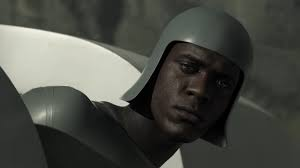
\includegraphics[scale=.7,rotate=-18]{Padre.jpg}\caption{La niñera}\\
         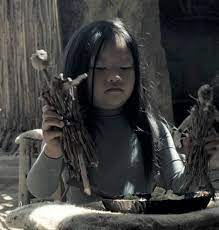
\includegraphics[scale=.4,rotate=8]{Vita, la chillona.jpg}{\caption{La chillona}}
         
           
         
\end{document}
